\newtheorem{proposition}{Proposition}
\newtheorem{lemma}{Lemma}
\newtheorem{assumption}{Assumption}

\chapter{Flexible generative modelling of varying dimensionality data}
\label{ch:tddm}

So far in this thesis we have described how to train a flexible diffusion model which can be conditioned on any subset of its components at test time, and how to adapt such a model to enable flexible generative modelling of high-dimensional video data with bounded compute resources. In this section we explore how to enable flexible generative modelling in another scenario: when the data $\rvx$ that we wish to model has unknown dimensionality. This can be an issue with molecular data, where the number of atoms may vary, or with video data, where the number of frames can vary. 

When defining a generative model over such data types, whether it is conditional or unconditional, it is necessary to model the number of dimensions along with the raw values of each of its dimensions (the state). Previous approaches to modelling such data have relied on first sampling the number of dimensions from the empirical distribution obtained from the training data, and then sampling data using a fixed dimension diffusion model (FDDM) conditioned on this number of dimensions~\cite{hoogeboom2022equivariant}. This works well for unconditional generative modelling. For conditional modelling, where the number of dimensions may depend on the observations, this approach does not apply and we are forced to first train an auxiliary model that predicts the number of dimensions given the observations~\cite{igashov2022equivariant}.

This approach to trans-dimensional generative modelling is fundamentally limited due to the complete separation of dimension generation and state value generation. A particular limitation is in the common use-case of conditional sampling from an unconditional diffusion model discussed in \cref{sec:other-methods-for-conditional-sampling}. Here, an unconditional diffusion model is trained that end-users can then easily and cheaply adapt to their task of interest through conditioning~\cite{song2020score, dhariwal2021diffusion, clip_guided_diffusion, zhang2023towards} without needing to perform any further training or fine-tuning of the model. In an FDDM, there is no way for the guidance to appropriately guide the dimension of the generated datapoint. This can lead to incorrect generations for datasets where the dimension greatly affects the nature of the datapoint created, which is common since e.g. small molecules have completely different properties to large molecules.

To generate data of varying dimensionality, we propose a jump diffusion based generative model that jointly generates both the dimension and the state. Our model can be seen as a unification of diffusion models which generate all dimensions in parallel with autoregressive type models which generate dimensions sequentially. We derive the model through constructing a forward noising process that adds noise and removes dimensions and a reverse generative process that adds dimensions while removing noise. We depict both processes in \cref{fig:tddm-fig1}. We derive the optimum reverse generative process as the time-reversal of the forward noising process and derive a novel learning objective to learn this reverse process from data. We demonstrate the advantages of our method on molecular and video datasets finding our method achieves superior guided generation performance and produces more representative data interpolations across dimensions.

\begin{figure}
    \centering
    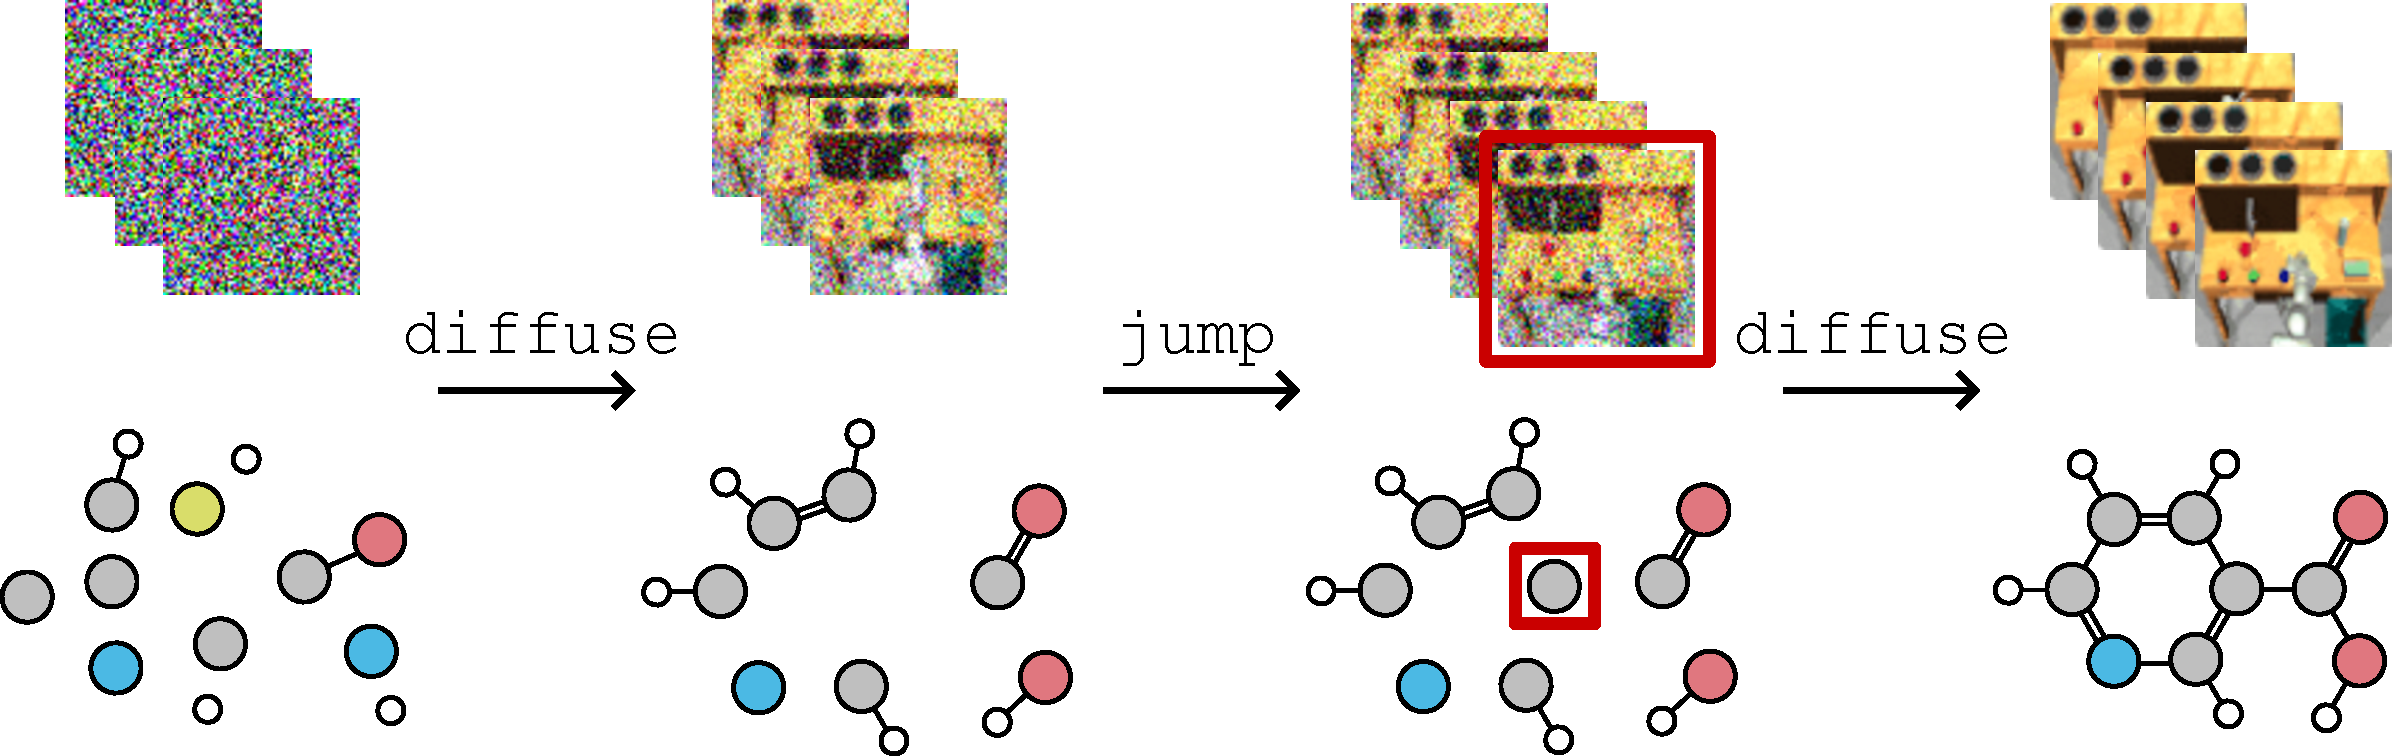
\includegraphics[width=\textwidth]{figs/tddm/fig1.pdf}
    \caption{Illustration of the jump diffusion generative process on videos and molecules. The generative process consists of two parts: a diffusion part which denoises the current set of frames (or atoms) and a jump part which adds on a suitable number of new frames (or atoms) such that the final generation is a clean synthetic datapoint of an appropriate size.
    }
    \label{fig:tddm-fig1}
\end{figure}


\section{Trans-dimensional diffusion model}
Instead of working with fixed dimension datapoints, we will instead assume our datapoints consist of a variable number of components. A datapoint $\mX$ consists of $n$ components each of dimension $d$. For ease of notation, each datapoint will explicitly store both the number of components, $n$, and the state values, $\rvx$, giving $\mX = (n, \rvx)$. Since each datapoint can have a variable number of components from $n=1$ to $n=N$, our overall space that our datapoints live in is the union of all these possibilities, $\mX \in \gX = \bigcup_{n=1}^N \{n \} \times \mathbb{R}^{nd}$. For example, for a varying size point cloud dataset, components would refer to points in the cloud, each containing $(x,y,z)$ coordinates giving $d=3$ and the maximum possible number of points in the cloud is $N$.

Broadly speaking, our approach will follow the same framework as previous diffusion models. We will first define a forward noising process that both corrupts state values with Gaussian noise and progressively deletes dimensions.
We then learn an approximation to the time-reversal giving a reverse generative process that simultaneously denoises whilst also progressively adding dimensions back until a synthetic datapoint of appropriate dimensionality has been constructed.

\paragraph{Notation}
In this chapter we will make two small modifications to how we describe marginals and conditionals of the forward process. First, we will more explicitly label the timesteps of each marginal and conditional distribution so that e.g. $q_t(\rvx_t)$ denotes what we previously called $q(\rvx_t)$ and $q_{t|0}(\rvx_t|\rvx)$ denotes what we previously called $q(\rvx_t|\rvx)$. Second, given that the forward process is now operating over $\mX_t \in \gX$ instead of $\rvx_t \in \mathbb{R}^{d}$, such marginal distributions can similarly be over $\mX_t$ instead of $\rvx_t$. We can therefore view the forward process as defining joint distributions of the form $q_{0,t_1,\ldots,t_n}(\mX,\mX_{t_1},\ldots,\mX_{t_n}) = q_{0,t_1,\ldots,t_n}(\rvx,n,\rvx_{t_1},n_{t_1},\ldots,\rvx_{t_n},n_{t_n})$ and any associated marginals and conditionals. This lets us consider distributions of the form $q_t(\rvx_t|n_t)$, which e.g. are conditional on the number of components $n_t$ but not on the data values $\rvx_t$.

\subsection{Forward process}
\label{sec:tddm-jump-diff-proc}

Our forward and reverse processes will be defined through jump diffusions. A jump diffusion process has two components, the diffusion part and the jump part. Between jumps, the process evolves according to a standard SDE. When a jump occurs, the process transitions to a different dimensional space with the new value for the process being drawn from a transition kernel $K_t(\mV | \mX_t): \gX \times \gX \rightarrow  \mathbb{R}_{\geq 0}$. Letting $\mV = (m, \rvv)$, the transition kernel satisfies $\sum_m \int_\rvv K_t(m, \rvv | \mX_t) \rmd \rvv = 1$ and $\int_\rvv K_t(m=n, \rvv | \mX_t) \rmd \rvv = 0$. The rate at which jumps occur (jumps per unit time) is given by a rate function $\lambda(\mX_t, t): \mathcal{X} \rightarrow \mathbb{R}_{\geq 0}$. 
We can describe a jump diffusion in terms of an infinitesimal timestep $\rmd t$. For the forward process we call the transition kernel $\ftk_t(\mV|\mX_t)$ and rate function $\forwardrate(\mX_t, t)$. We will give their precise definitions shortly. Given this notation, we write the forward jump diffusion as
\begin{align}
    \textbf{Jump} \hspace{1cm} & \mX_t' = \begin{cases}
        \mX_t & \text{with probability } 1 - \forwardrate(\mX_t, t) \rmd t \\
        \mV \sim \ftk_t( \mV |\mX_t) & \text{with probability } \forwardrate(\mX_t, t) \rmd t
    \end{cases}  \label{eq:tddm-forward-jump} \\
    \textbf{Diffusion} \hspace{1cm} &\rvx_{t+ \rmd t} = \rvx'_t + \rvb(\rvx'_t, t) \rmd t + g(t) \rmd \brown_t \hspace{1cm} n_{t+\rmd t} = n_t'
     \label{eq:tddm-forward-diffusion}
\end{align}
with $\mX_t \triangleq (n_t, \rvx_t)$ and $\mX_{t+\rmd t} \triangleq (n_{t+\rmd t}, \rvx_{t + \rmd t})$ and $\rmd \brown_t$ being a Brownian motion increment on $\mathbb{R}^{n_t'd}$.

With the jump diffusion formalism in hand, we can now construct our forward noising process. We will use the diffusion part to corrupt existing state values with Gaussian noise and the jump part to destroy dimensions. For the diffusion part, we use the variance-preserving diffusion SDE introduced in \cref{ch:diffusion}~\cite{ho2020denoising, song2020score} so $\rvb(\rvx_t, t) = -\frac{1}{2}g(t)^2 \rvx_t$.

When a jump occurs in the forward process, one component of the current state will be deleted.
For example, one point in a point cloud or a single frame in a video is deleted. The rate at which these deletions occur is set by a user-defined forward rate $\smash{\forwardrate}(\mX_t, t)$. To formalise the deletion, we need to introduce some more notation. We let $\delidxdist(i | n_t)$ be a user-defined distribution over which component of the current state to delete. We also define $\text{del}: \mathcal{X} \times \mathbb{N} \rightarrow \mathcal{X}$ to be the deletion operator that deletes a specified component. Specifically, $(n_t-1, \rvv) = \text{del}((n_t, \rvx_t), i)$ where $\rvv \in \mathbb{R}^{(n-1)d}$ has the same values as $\rvx_t \in \mathbb{R}^{nd}$ except for the $d$ values corresponding to the $i$th component which have been removed. 
We can now define the forward jump transition kernel as $\ftk_t(\mV | \mX_t) = \sum_{i=1}^n \delidxdist (i | n_t) \updelta_{\text{del}(\mX_t, i)}(\mV)$. We note that only one
component is ever deleted at a time meaning $\ftk_t(m, \rvv | \mX_t) = 0$ for $m \neq n_t - 1$. Further, the choice of $\delidxdist(i | n_t)$ will dictate the behaviour of the reverse generative process. If we set $\delidxdist(i | n_t) = \mathbb{I}\{i=n_t\}$ then we only ever delete the final component and so in the reverse generative direction, datapoints are created additively, appending components onto the end of the current state. Alternatively, if we set $\delidxdist(i | n_t) = 1/n_t$ then components are deleted uniformly at random during forward corruption and in the reverse generative process, the model will need to pick the most suitable location for a new component from all possible positions.

The forward noising process is simulated from $t=0$ to $t=T$ and should be such that at time $t=T$, the marginal probability $q_T(\mX_T)$ should be close to a reference measure $\pref(\mX_T)$ that can be sampled from, similarly to the standard approximation of $q_T(\rvx_T)$ with a Gaussian in the fixed-dimensional diffusion setting. 
We set $\pref(\mX_T) = \mathbb{I} \{ n_T = 1\} \mathcal{N}(\rvx_T; 0, I_{d})$ where $\mathbb{I} \{ n_T = 1\}$ is $1$ when $n_T=1$ and $0$ otherwise. To be close to $\pref$, for the jump part, we set $\forwardrate$ high enough such that at time $t=T$ there is a high probability that all but one of the components in the original datapoint have been deleted. For simplicity, we also set $\forwardrate$ to depend only on the current dimension $\forwardrate(\mX_t, t) = \forwardrate(n_t, t)$ with $\forwardrate(n_t=1, t) = 0$ so that the forward process stops deleting components when there is only $1$ left. In our experiments in \cref{sec:tddm-experiments} we demonstrate the trade-offs between different rate schedules in time. For the diffusion part, we use standard $g(t)$ schedules which ensure that we are close to $\mathcal{N}(\rvx_t; 0, I_{d})$.

\subsection{Reverse process}
The reverse generative process will simultaneously denoise and add dimensions back in order to construct the final datapoint. Its drift term corresponds to that of a standard reverse diffusion SDE from \cref{ch:diffusion}, consisting of the sum of the forward drift term and a scaled score function. We will call the reverse rate function $\backwardrate(\mX_t, t)$, the reverse transition kernel $\btk_t(\mV | \mX_t)$, the reverse drift term $\backwarddrift(\mX_t, t)$ and the backwards diffusion coefficient $\backwarddiffcoeff(t)$ so write the reverse jump diffusion as
\begin{align}
    \label{eq:tddm-reverse-jump}
    \textbf{Jump} \hspace{.4cm} & \mX_t' = \begin{cases}
        \mX_t & \text{with probability } 1 - \backwardrate(\mX_t, t) \rmd t \\
        \mV \sim \btk_t( \mV |\mX_t) & \text{with probability } \backwardrate(\mX_t, t) \rmd t
    \end{cases} 
    \\
    \label{eq:tddm-reverse-diffusion}
    \textbf{Diffusion} \hspace{.4cm} &\rvx_{t+ \rmd t} = \rvx'_t + \backwarddrift(\rvx'_t, t)
    % \left(b(t)\rvx_t + g(t)^2 \rvs_\theta(\mX, t) \right) 
    \rmd t + \backwarddiffcoeff(t) \rmd \brown_t \hspace{.5cm} n_{t+\rmd t} = n_t'
\end{align}
We would now like to specify the form of $\backwardrate(\mX_t, t)$, $\btk_t(\mV|\mX_t)$, and $\backwarddrift(\mX_t, t)$ which ensure that the reverse process is the time-reversal of the forward process. 
% In order to find the time-reversal of the forward process, we must first introduce some notation to describe $\btk_t(\mV | \mX)$.
$\btk_t(\mV | \mX_t)$ should undo the forward deletion operation. Since $\ftk_t(\mV | \mX_t)$ chooses a component and then deletes it, $\btk_t(\mV | \mX_t)$ will need to generate the state values for a new component, decide where the component should be placed and then insert it at this location. 
Our new component will be denoted $\yadd \in \mathbb{R}^{d}$. 
The insertion operator is defined as $\text{ins}: \gX \times \mathbb{R}^{d} \times \mathbb{N} \rightarrow \gX$. It takes in the current value $\mX_t$, the new component $\yadd$ and an index $i \in \{1, \dots, n+1\}$ and inserts $\yadd$ into $\mX_t$ at location $i$ such that the resulting value $\mV = \text{ins}(\mX_t, \yadd, i)$ has $\text{del}(\mV, i) = \mX_t$.
We denote the joint conditional distribution over the newly added component and the index at which it is inserted as $\autonet_t(\yadd, i | \mX_t)$.
We therefore have $\btk_t(\mV | \mX_t) = \int_{\yadd} \sum_{i=1}^{n+1}  \autonet_t(\yadd, i | \mX_t) \updelta_{\text{ins}(\mX_t, \yadd, i)}(\mV) \rmd \yadd$. Noting that only one component is ever added at a time, we have $\btk_t(m, \rvv | \mX_t) = 0$ for $m \neq n+1$. 

This reverse process formalism can be seen as a unification of diffusion models with autoregressive models. The diffusion part $\backwarddrift$ denoises the current set of components in parallel, whilst the autoregressive part $\autonet_t(\yadd, i | \mX_t)$ predicts a new component and its location. $\backwardrate(\mX_t, t)$ is the glue between these parts controlling when and how many new components are added during generation.

The following proposition states the values for $\backwarddrift(\mX_t, t)$, $\backwarddiffcoeff(t)$, $\backwardrate(\mX_t, t)$ and $A_t(\yadd, i | \mX_t)$ which ensure that the reverse process is the time-reversal of the forward process.
\begin{proposition}
\label{prop:time_reversal}
The time reversal of a forward jump diffusion process given by transition kernel $\sum_{i=1}^n \delidxdist(i | n_t) \updelta_{\textup{del}(\mX_t, i)}(\mV)$, drift $\rvb(\rvx_t, t)$, diffusion coefficient $g(t)$, and rate $\forwardrate(n_t, t)$ is given by a jump diffusion process with drift term $\backwarddrift$, diffusion coefficient $\backwarddiffcoeff^*(t)$, transition kernel $\int_{\yadd} \sum_{i=1}^{n+1}  \autonet^*_t(\yadd, i | \mX_t) \updelta_{\textup{ins}(\mX_t, \yadd, i)}(\mV) \rmd \yadd$, and rate $\backwardrate^*(\mX_t, t)$ as defined below:
\begin{align}
    &\backwarddrift^*(\mX_t, t) = \rvb(\mX_t, t) - g(t)^2 \nabla_{\rvx_t} \log q_t(\mX_t), \qquad \backwarddiffcoeff^*(t) = g(t),\\
    & \backwardrate^*(\mX_t, t) = \forwardrate(n_t+1, t) \frac{ \sum_{i=1}^{n_t+1} \delidxdist(i | n_t+1) \int_{\yadd} q_t(\textup{ins}(\mX_t, \yadd, i)) \rmd \yadd }{q_t(\mX_t)},\\
    & \autonet_{t}^*( \yadd, i | \mX_t) \propto q_{t}(\textup{ins}(\mX_t, \yadd, i) ) \delidxdist(i| n_t+1).
\end{align}
\end{proposition}
This dissertation focuses on how jump diffusion process enables new conditional generation tasks rather than the mathematical foundations of jump diffusion so we refer to Appendix A of \citet{campbell2024trans} for a proof. The expressions for $\backwarddrift^*$ and $\backwarddiffcoeff^*(t)$ are the same as for a standard diffusion except for replacing $\nabla_{\rvx} \log q_t(\rvx_t)$ with $\nabla_{\rvx_t} \log q_t(\mX_t) = \nabla_{\rvx_t} \log q_t(\rvx_t | n_t)$ which is simply the score in the current dimension.
The expression for $\backwardrate^*$ can be understood intuitively by noting that the numerator in the probability ratio is the probability that at time $t$, given a deletion occurs, the forward process will arrive at $\mX_t$. If this is higher than the raw probability at time $t$ that the forward process is at $\mX_t$ (the denominator) then we should have high $\backwardrate^*$ because $\mX_t$ is likely the result of a deletion of a larger datapoint.
Finally the optimum $\autonet^*_t(\yadd, i | \mX_t)$ is simply the conditional distribution of $\yadd$ and $i$ given $\mX_t$ when the joint distribution over $\yadd, i, \mX_t$ is given by $q_{t}(\text{ins}(\mX_t, \yadd, i) ) \delidxdist(i| n+1)$. 

\subsection{Objective for learning the reverse process}
The true $\backwarddrift^*$, $\backwardrate^*$ and $\autonet_t^*$ are unknown so we need to learn approximations to them, $\backwarddrift_\theta$, $\backwardrate_\theta$ and $\autonet_t^\theta$. 
To parameterise the diffusion component of the reverse process, we can follow the procedure used in a standard diffusion model to learn the score function $\rvs_\theta(\mX_t, t) \approx \nabla_{\rvx_t} \log q_t(\mX_t)$. To parameterise the jump component, which relies on an unknown optimal rate $\backwardrate^*$ and unknown distribution $\autonet_t^*$, we will need a novel objective to learn approximations to $\backwardrate_\theta$ and $\autonet_t^\theta$.

As we showed in \cref{ch:diffusion}, the standard diffusion score matching loss can be derived from maximising an evidence lower bound on the model probability for $ \mathbb{E}_{\pdata(\rvx)} [ \log p_\theta(\rvx) ]$ \cite{song2021maximum}.
We present here an equivalent loss to learn all of $\rvs_\theta$, $\smash{\backwardrate_\theta}$ and $\autonet_t^\theta$ for our jump diffusion process by leveraging the results of \citet{benton2022denoising,cheridito2005equivalent}, referring to Appendix A of \citet{campbell2024trans} for its rigorous derivation. Before presenting this loss, we first introduce some notation. Our objective for $s_\theta(\mX_t, t)$ will resemble denoising score matching (as in \cref{eq:exp-diffusion-loss-all-sigma} of \cref{sec:diffusion-training}) but instead involve the conditional score $\nabla_{\rvx_t} \log q_{t|0}(\mX_t | \mX) = \nabla_{\rvx_t} \log q_{t|0}(\rvx_t | \mX, n_t)$. This is difficult to calculate directly due to a combinatorial sum over the different ways the components of $\mX$ can be deleted to get to $\mX_t$. We avoid this problem by equivalently conditioning on a mask variable $M_t \in \{0, 1\}^{n}$ that is 0 for components of $\mX$ that have been deleted to get to $\mX_t$ and 1 for components that remain in $\mX_t$. This makes our denoising score matching target easy to calculate: $\nabla_{\rvx_t} \log q_{t|0}(\rvx_t | \mX, n_t, M_t) = \frac{\alpha(t) M_t(\rvx) - \rvx_t}{\sigma(t)^2}$. Here $M_t(\rvx)$ is the vector removing any components in $\rvx$ for which $M_t$ is $0$, thus $M_t(\rvx)$ and $\rvx_t$ have the same dimensionality. We now state our full objective.

\begin{proposition}
\label{prop:elbo}
For the reverse generative jump diffusion process starting at $\pref(\mX_T)$ and finishing at $ q_0^\theta(\mX)$, an evidence lower bound on the model log-likelihood $ \mathbb{E}_{\rvx \sim \pdata(\cdot)} [ \log p_\theta(\rvx) ]$ is given by
\begin{align}
    \label{eq:tddm-elbo}
    \mathcal{L}_\text{JD}(\theta) = -\frac{T}{2} \mathbb{E}\Big[& g(t)^2 \norm{s_\theta(\mX_t, t) - \nabla_{\rvx_t} \log q_{t|0}(\rvx_t | \mX, n_t, M_t)   }^2 \Big] + \\
    \nonumber
    T \mathbb{E} \Big[& - \backwardrate_\theta(\mX_t, t) + \forwardrate (n_t, t) \log \backwardrate_\theta(\mV, t) + \forwardrate(n_t, t) \log \autonet_{t}^\theta(\xadd_t, i | \mV) \Big] \\
    \nonumber
    + C,
\end{align}
where expectations are w.r.t. $\mathcal{U}(t; 0, T) q_{0,t}(\mX, \mX_t, M_t) \delidxdist(i | n_t) \updelta_{\textup{del}(\mX_t, i)} (\mV)$, $C$ is a constant term independent of $\theta$ and $\mX_t = \text{ins}(\mV, \xadd_t, i)$.
This evidence lower bound is equal to the log-likelihood when $\backwarddrift_\theta = \backwarddrift^*$, $\backwardrate_\theta = \backwardrate^*$ and $A_t^\theta = A_t^*$.
\end{proposition}

We now examine the objective to gain an intuition into the learning signal.
Our first term in \cref{eq:tddm-elbo} is an $L_2$ regression to a score function that, as we have seen, is a scaled vector between $\rvx_t$ and $\alpha(t) M_t(\rvx)$. As the solution to an $L_2$ regression problem is the conditional expectation of the target, $\rvs_\theta(\mX_t, t)$ will learn to predict vectors pointing towards $\rvx$ averaged over the possible correspondences between dimensions of $\rvx_t$ and dimensions of $\rvx$.
Thus, during sampling, $\rvs_\theta(\mX_t, t)$ provides a suitable direction to adjust the current value $\mX_t$ taking into account the fact $\mX_t$ represents only a noisy subpart of a clean whole $\mX$. Comparing this objective with the form introduced in \cref{ch:diffusion}, we see that the weighting factor $\lambda^\rvs / u(t)$ is set to $g(t)^2$ to achieve this lower-bound on the data likelihood. In our experiments we will adjust this weighting factor, following \citet{song2020score} to improve the perceptual quality as discussed in \cref{sec:diffusion-perceptual-quality}. See \cref{sec:tddm-ApdxTrainingObjective} for full details.

The second line of \cref{eq:tddm-elbo} gives a learning signal for $\backwardrate_\theta$ and $\autonet_{t}^\theta$.
For $\autonet_{t}^\theta$, we simply have a maximum likelihood objective, predicting the missing part of $\mX_t$ (i.e.~$\xadd_t$) given the observed part of $\mX_t$ (i.e.~$\mV$).
The signal for $\backwardrate_\theta$ comes from balancing two terms: $-\backwardrate_\theta(\mX_t, t)$ and $\forwardrate(n_t, t) \log \backwardrate_\theta(\mV, t)$ which encourage the value of $\backwardrate_\theta$ to move in opposite directions. For a new test input $\mZ$, $\backwardrate_\theta(\mZ, t)$'s value needs to trade off between the two terms by learning the relative probability between $\mZ$ being the entirety of a genuine sample from the forward process, corresponding to the $\backwardrate_\theta(\mX_t, t)$ term in \cref{eq:tddm-elbo}, or $\mZ$ being a substructure of a genuine sample, corresponding to the $\backwardrate_\theta(\mV, t)$ term in \cref{eq:tddm-elbo}. The optimum trade-off is found exactly at the time reversal $\backwardrate^*$ as shown in Appendix A.5 of \citet{campbell2024trans}.

Similarly to a standard diffusion model, we optimise $\mathcal{L}_\text{JD}(\theta)$ using stochastic gradient ascent. We generate training batches by first sampling $t \sim \mathcal{U}(0, T)$, $\mX \sim \pdata(\cdot)$ and then computing $\mX_t$ from  the forward process. This can be done analytically for the $\forwardrate(n_t, t)$ functions used in our experiments. We first sample $n_t$ by analytic integration of the dimension deletion Poisson process with time inhomogeneous rate $\forwardrate(n_t, t)$. We then add Gaussian noise independently to each dimension under $q_{t|0}(\rvx_t | \mX, n_t, M_t)$ using a randomly drawn mask variable $M_t$. See \cref{sec:tddm-ApdxTrainingObjective} for further details on the efficient evaluation of our objective. 

\subsection{Parameterisation}

We use neural networks to parameterise all of $\rvs_\theta(\mX_t, t)$, $\autonet_t^\theta(\yadd, i | \mX_t)$ and $\backwardrate_\theta(\mX_t, t)$. In practice, we have a single backbone network suited to the problem of interest e.g. a Transformer \cite{vaswani2017attention}, an EGNN \cite{satorras2021n} or a U-Net \cite{ronneberger2015u} onto which we add prediction heads for $\rvs_\theta(\mX_t, t)$, $\autonet_t^\theta(\yadd, i | \mX_t)$ and $\backwardrate_\theta(\mX_t, t)$. $\rvs_\theta(\mX_t, t)$ outputs a vector in $\mathbb{R}^{n_t d}$. $\autonet_t^\theta(\yadd, i | \mX_t)$ outputs a distribution over $i$ and mean and standard deviation statistics for a Gaussian distribution over $\yadd$. Finally, having $\backwardrate_\theta(\mX_t, t) \in \mathbb{R}_{\geq 0}$ be the raw output of a neural network can cause optimisation issues due to the optimum $\backwardrate^*$ including a probability ratio which can take on very large values. Instead, we learn a component prediction network $p^\theta_{0|t}(n | \mX_t)$ that predicts the number of components in $\mX$ given $\mX_t$. To convert this into $\backwardrate_\theta(\mX_t, t)$, we show in \cref{prop:backwardrateparam} how the optimum $\backwardrate^*(\mX_t, t)$ is an analytic function of the true $q_{0|t}(n | \mX_t)$. We then plug $q_{0|t}(n | \mX_t)$ into \cref{prop:backwardrateparam} to obtain an approximation of $\backwardrate^*(\mX_t, t)$.
\begin{proposition} We have
    \label{prop:backwardrateparam}
    \begin{equation}\label{eq:backwardrateparam}
        \backwardrate^*(\mX_t, t) = \forwardrate(n_t+1, t) \sum_{n=1}^N \frac{q_{t|0}(n_t + 1 | n)}{q_{t|0}(n_t | n)} q_{0|t}(n | \mX_t),
    \end{equation}
    where $\mX_t = (n_t, \rvx_t)$ and $q_{t|0}(n_t + 1 | n)$ and $q_{t|0}(n_t | n)$ are both easily calculable distributions from the forward dimension deletion process.
\end{proposition}



\subsection{Sampling}

\begin{algorithm}[t]
\caption{Sampling with the generative process.}
\begin{algorithmic}[1] % The [1] option enables line numbering
\State $t \leftarrow T$
\State $\mX' \sim \pref(\cdot) = \mathbb{I}\{ n'=1\} \mathcal{N}(\rvx'; 0, I_{d})$
\While{$t > 0$}
    \State $u \sim \mathcal{U}(0, 1)$
    \If{$u < \backwardrate_\theta(\mX', t) \updelta t$}
        \State $\xadd, i \sim \autonet_{t}^\theta(\xadd, i | \mX')$
        \State $\mX' \leftarrow \text{ins}(\mX', \xadd, i)$
    \EndIf
    \State $\epsilon \sim \mathcal{N}(0, I_{nd})$
    \State $\rvx' \leftarrow \rvx' - \backwarddrift_\theta(\mX', t) \updelta t + g(t) \sqrt{\updelta t} \epsilon$
    \State $\mX' \leftarrow (n', \rvx')$
    \State $t \leftarrow t - \updelta t$
\EndWhile
\end{algorithmic}
\label{alg:backwardsampling}
\end{algorithm}

To sample the generative process, we numerically integrate the learned reverse jump diffusion process using time-step  $\updelta t$. Intuitively, it is simply the standard continuous time diffusion sampling scheme \cite{song2020score} but at each timestep we check whether a jump has occurred and if it has, sample the new component and insert it at the chosen index as explained by \cref{alg:backwardsampling}.

\subsection{Trans-dimensional reconstruction guidance} \label{sec:tddm-reconstruction-guidance}
We now detail how we transport the reconstruction guidance method from \cref{sec:reconstruction-guidance} to the trans-dimensional case to enable conditional sampling from unconditional jump diffusion models. Similarly to \cref{sec:reconstruction-guidance} we will condition on $n_\rvy$ components at indices $\gY$ whose values we denote $\rvy = \rvx[\gY]$.
Naturally, conditioning on $\rvy$ will be informative about the data values $\rvx$ and also about the number of components in the data, $n$. The dependence of the number of components $n$ of the observations $\mY$ comes both in the form of a bound $n \geq n_\rvy$ and in any data-dependent relationships between $n$ and the observed values $\rvy$.

To perform reconstruction guidance, we will assume that we know a correspondence between components of $\rvy$ and components of $\rvx_t$. Since we demonstrate reconstruction guidance on molecular data where the set of components is permutation invariant, we can simply match the first $n_\rvy$ components in $\rvx_t$ to the $n_\rvy$ components in $\rvy$. We will implicitly condition on this correspondence whenever we condition on $\rvy$.

In principle, making a conditional model involves modifying all of the score function estimator $\rvs_\theta$, the reverse rate function $\backwardrate_\theta$ and the autoregressive conditional distribution $\autonet_t^\theta$ to be conditional on $\rvy$ (and the assumed correspondence). In practice, we found that we only needed to modify the score function estimate to obtain good results. Analogously to \cref{sec:reconstruction-guidance}, we have $\rvs_\theta(\mX_t, t) \approx \nabla_{\rvx_t} q_{t|0} (\mX_t) = \nabla_{\rvx_t} q_{t|0} (\rvx_t, n_t)$ but need an approximation of $\nabla_{\rvx_t} q_{t|0} (\mX_t | \rvy )$. We derive one as
\begin{align}
    \nabla_{\rvx_t} q_{t|0} (\mX_t | \rvy ) = \underbrace{\nabla_{\rvx_t} q_{t|0} (\mX_t)}_{\approx \rvs_\theta(\mX_t, t)} + \underbrace{\nabla_{\rvx_t} q_{0|t} (\rvy | \mX_t)}_\text{intractable likelihood gradient}.
\end{align}
The intractable likelihood gradient can be estimated using the score function of a Gaussian approximation as in \cref{sec:reconstruction-guidance} leading to the estimate
\begin{equation} \label{eq:tddm-guidance-term}
    \nabla_{\rvx_t} \log q_{0|t}(\rvy | \mX_t) \approx - \frac{\alpha(t)^2}{2\sigma(t)^2} \nabla_{\rvx_t} \norm{\rvy - \predx_\theta(\mX_t, t)[\gY] }^2_2.
\end{equation}
where $\predx_\theta(\mX_t, t)[\gY]$ are the predictions of $\rvx$ corresponding to our observed components. This can be computed by differentiating through the score network $\rvs_\theta$.  Note, though, that there is a slight abuse of notation in \cref{eq:tddm-guidance-term} as, for large $t$, $\rvx_t$ can have fewer components than $\rvy$ in which case we modify the squared L2 distance term in \cref{eq:tddm-guidance-term} to be between only the components of $\rvy$ and predictions of $\rvx$ that exist in $\rvx_t$.

Including the guidance weight $w$ introduced in \cref{sec:reconstruction-guidance}, which we set to $w = 1$ in our experiments, our final score function estimate is
\begin{equation} \label{eq:tddm-guidance-score}
    \nabla_{\rvx_t} q_{t|0} (\mX_t | \rvy ) = \nabla_{\rvx_t} q_{t|0} (\mX_t) - \frac{w \cdot \alpha(t)^2}{2\sigma(t)^2} \nabla_{\rvx_t} \norm{\rvy - \predx_\theta(\mX_t, t)[\gY] }^2_2.
\end{equation}

As mentioned, we approximate $\backwardrate^*(\mX_t | \mY, t)$ and $\autonet_t^*(\yadd, i | \mX_t, \mY)$, with their unconditional forms $\backwardrate_\theta(\mX_t, t)$ and $\autonet_t^\theta(\yadd, i | \mX_t)$. We find this approximation still leads to valid generations because the guidance of the score network $s_t^\theta$, results in $\mX_t$ containing the conditioning information which in turn leads to $\backwardrate_\theta(\mX_t)$ guiding the number of components in $\mX_t$ to be consistent with the conditioning information too as verified in our experiments. Further, any errors in the approximation for $\autonet_t^\theta(\yadd, i | \mX_t)$ are fixed by further applications of the guided score function, highlighting the benefits of our combined autoregressive and diffusion based approach.



\section{Related work}

Our method jointly generates both dimensions and state values during the generative process whereas prior approaches \cite{hoogeboom2022equivariant, igashov2022equivariant} are forced to first sample the number of dimensions and then run the diffusion process in this fixed dimension. When diffusion guidance is applied to these unconditional models \cite{weiss2023guided, zhang2023towards}, users need to pick by hand the number of dimensions independent of the conditioning information even though the number of dimensions can be correlated with the conditioning parameter.

Instead of automatically learning when and how many dimensions to add during the generative process, previous work focusing on images \cite{jing2022subspace, zhang2022dimensionality} hand pick dimension jump points such that the resolution of images is increased during sampling and reaches a certain pre-defined desired resolution at the end of the generative process. Further, rather than using any equivalent of $\autonet_t^\theta$, the values for new dimensions are simply filled in with Gaussian noise. These approaches mainly focus on efficiency rather than flexible generation as we do here.


The first term in our learning objective in \cref{prop:elbo} corresponds to learning the continuous part of our process (the diffusion) and the second corresponds to learning the discrete part of our process (the jumps). The first term can be seen as a trans-dimensional extension of standard denoising score matching \cite{vincent2011connection} whilst the second bears similarity to the discrete space ELBO derived in \cite{campbell2022continuous}.

Finally, jump diffusions also have a long history of use in Bayesian inference, where one aims to draw samples from a trans-dimensional target posterior distribution based on an unnormalised version of its density \cite{grenander1994representations}: an ergodic jump diffusion is designed which admits the target as the invariant distribution \cite{grenander1994representations,phillips1995bayesian,miller1997automatic}. The invariant distribution is not preserved when time-discretising the process.
However, it was shown in  \cite{green1995reversible,green2003trans} how general jump proposals could be built and how this process could be ``Metropolized'' to obtain a discrete-time Markov process admitting the correct invariant distribution, yielding the popular Reversible Jump Markov Chain Monte Carlo algorithm.
Our setup differs significantly as we only have access to samples in the form of data, not an unnormalised target.


\section{Experiments} \label{sec:tddm-experiments}

\subsection{Molecules}
We now show how our model provides significant benefits for diffusion guidance and interpolation tasks. We model the QM9 dataset \cite{ruddigkeit2012enumeration, ramakrishnan2014quantum} of 100\,000 varying size molecules. Following \cite{hoogeboom2022equivariant}, we consider each molecule as a 3-dimensional point cloud of atoms, each atom having the features: $(x,y,z)$ coordinates, a one-hot encoded atom type, and an integer charge value. Bonds are inferred from inter-atomic distances. We use an EGNN \cite{satorras2021n} backbone with three heads to predict $\smash{\rvs_\theta}$, $\smash{p_{0|t}^\theta(n | \mX_t)}$, and $\smash{\autonet_t^\theta}$. We uniformly delete dimensions, $K^{\text{del}}(i | n) = 1/n$, and since a point cloud is permutation invariant, $\smash{\autonet_t^\theta(\yadd | \mX_t)}$ need only predict new dimension values. We set $\smash{\forwardrate}$ to a constant value except for $t < 0.1T$, where we set it to zero. This ensures that all dimensions are added with enough generation time remaining for the diffusion process to finalise all state values. 

We visualise sampling from our learned generative process in \cref{fig:tddm-uncond_chain_vis}; note how the process jointly creates a suitable number of atoms whilst adjusting their positions and identities. Before moving on to apply diffusion guidance, which is the focus of our experiments, we first verify our unconditional sample quality in \cref{tab:uncond_mol} and find we perform comparably to the results reported in \citet{hoogeboom2022equivariant} which use an FDDM. We ablate our choice of $\smash{\forwardrate}$ by comparing with setting $\smash{\forwardrate}$ to a constant for all $t$ (giving ``const $\forwardrate$'') and with setting $\smash{\forwardrate(n_t, t)}=0$ for $t<0.9T$ rather than just for $t<0.1T$ (giving ``$\smash{\forwardrate_{t<0.9T} = 0}$''). We find that the constant $\smash{\forwardrate}$ performs worse due to the occasional component being added late in the generation process without enough time for the diffusion process to finalise its value. We find the $\smash{\forwardrate_{t<0.9T} = 0}$ setting to have satisfactory sample quality however this choice of $\smash{\forwardrate}$ introduces issues during diffusion guided generation as we see next. Finally, we ablate the parameterisation of \cref{prop:backwardrateparam} by learning $\backwardrate_\theta(\mX_t, t) \in \mathbb{R}$ directly as the output of a neural network head. We find that this reduces sample quality due to the more well-behaved nature of the target, $p_{0|t}^\theta(n | \mX_t)$ when using \cref{prop:backwardrateparam}. We note pure autoregressive models perform significantly worse than diffusion based models as found by \citet{hoogeboom2022equivariant}.

\begin{figure}[t]
    \centering
    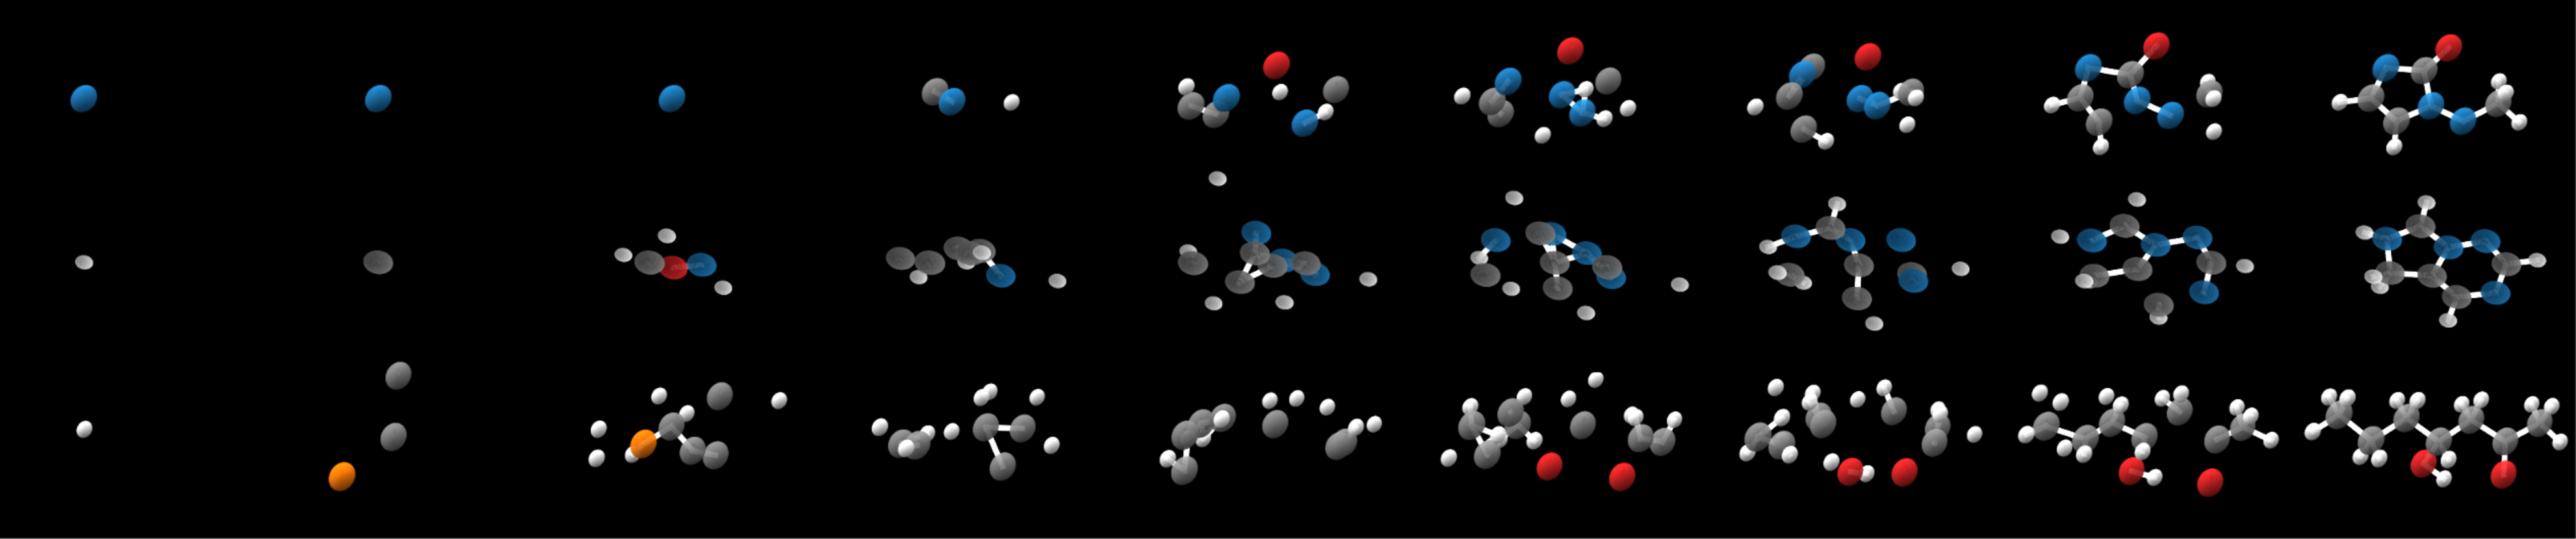
\includegraphics[width=\textwidth]{figs/tddm/genprog.pdf}
    \caption{Visualisation of the jump diffusion reverse process learned by our model trained on molecular data.}
    \label{fig:tddm-uncond_chain_vis}
\end{figure}


\begin{table}[t]
\caption{Evaluation of molecules generated unconditionally by our method and baselines. An atom is stable if it has the correct valency whilst a molecule is considered stable if all of its atoms are stable. Molecular validity is measured using RDKit~\citep{rdkit}. All methods use 1000 simulation steps and draw 10000 samples.}
\label{tab:uncond_mol}
\centering
\begin{tabular}{@{}lccc@{}}
\toprule
Method & \shortstack{\% Atom Stable ($\uparrow$)} & \shortstack{ \% Molecule Stable ($\uparrow$)} & \% Valid ($\uparrow$) \\ \midrule
FDDM \cite{hoogeboom2022equivariant} & $\mathbf{98.7}$ & $82.0$ & $91.9$  \\ \midrule
TDDM (ours) & $98.3$  & $\mathbf{87.2}$ & $\mathbf{92.3}$ \\
TDDM, const $\smash{\forwardrate}$ & $96.7$ & $79.1$ & $86.7$ \\
TDDM, $\smash{\forwardrate_{t<0.9T} = 0}$ & $97.7$ & $82.6$ & $89.4$ \\
TDDM w/o Prop. \ref{prop:backwardrateparam} & $97.0$ & $66.9$ & $87.1$ \\ \bottomrule
\end{tabular}
\end{table}
 

\subsubsection{Trans-dimensional reconstruction guidance}
\label{sec:mol_diff_guide}
We now apply reconstruction guidance as described in \cref{sec:tddm-reconstruction-guidance} to our unconditional model in order to generate molecules that contain a certain number of desired atom types, e.g. 3 carbons or 1 oxygen and 2 nitrogens. The distribution of molecule sizes changes depending on these conditions.

\begin{table}[tb]
\caption{Evaluation of conditional molecule generation for 10 conditioning tasks that each result in a different dimension distribution. We report dimension error as the average Hellinger distance between the generated and ground truth dimension distributions for that property as well as average sample quality metrics. Standard deviations are given across the 10 conditioning tasks. We report in bold values that are statistically indistinguishable from the best result at the $5\%$ level using a two-sided Wilcoxon signed rank test across the 10 conditioning tasks.}
\label{tab:cond_mol}
\centering
\begin{tabular}{@{}lcccc@{}}
\toprule
Method & \shortstack{Dimension \\ Error ($\downarrow$) } & \shortstack{ \% Atom \\ Stable ($\uparrow$)} & \shortstack{\% Molecule \\ Stable ($\uparrow$)} & \% Valid ($\uparrow$) \\ \midrule
FDDM & $0.511 {\scriptstyle \pm 0.19}$ & $93.5 {\scriptstyle \pm 1.1}$ & $31.3 {\scriptstyle \pm 6.3}$ & $65.2 {\scriptstyle \pm 10.3}$ \\ \midrule
TDDM (ours) & $\mathbf{0.134 {\scriptstyle \pm 0.076}}$ & $93.5 {\scriptstyle \pm 2.6}$ & $\mathbf{59.1 {\scriptstyle \pm 11}}$ & $\mathbf{74.8 {\scriptstyle \pm 9.3}} $ \\
 TDDM, const $\smash{\forwardrate}$ & $0.226 {\scriptstyle \pm 0.17}$ & $88.9 {\scriptstyle \pm 4.8}$   & $43.6 {\scriptstyle \pm 15}$ & $63.4 {\scriptstyle \pm 14}$ \\
 TDDM, $\smash{\forwardrate_{t<0.9T} = 0}$&  $0.390 {\scriptstyle \pm 0.38}$& $\mathbf{95.0 {\scriptstyle \pm 2.1}}$& $\mathbf{61.7 {\scriptstyle \pm 17}}$ & $\mathbf{77.8 {\scriptstyle \pm 13}} $ \\
 TDDM w/o \cref{prop:backwardrateparam} & $0.219 {\scriptstyle \pm 0.12} $ & $\mathbf{93.8 {\scriptstyle \pm 3.2}}$ & $55.0 {\scriptstyle \pm 19}$ & $73.8 {\scriptstyle \pm 13}$  \\ \bottomrule
\end{tabular}
\end{table}

We show our results in \cref{tab:cond_mol}. In order to perform reconstruction guidance on the FDDM baseline, we implement the model from \cite{hoogeboom2022equivariant} in continuous time and initialise the dimension from the empirically observed dimension distribution in the dataset.  This accounts for the case of an end user attempting to guide a unconditional model with access to no further information. We find that our method, TDDM, produces samples whose dimensions much more accurately reflect the true conditional distribution of dimensions given the conditioning information.
The $\forwardrate_{t<0.9T} = 0$ ablation on the other hand only marginally improves the dimension error over FDDM because all dimensions are added in the generative process at a time when $\mX_t$ is noisy and has little relation to the conditioning information. This highlights the necessity of allowing dimensions to be added throughout the generative process to gain the trans-dimensional diffusion guidance ability. The ablation with constant $\forwardrate$ has increased dimension error over TDDM as we find that when $\forwardrate > 0$ for all $t$, $\backwardrate_\theta$ can become very large when $t$ is close to 0 when the model has perceived a lack of dimensions. This occasionally results in too many dimensions being added hence an increased dimension error. Not using the \cref{prop:backwardrateparam} parameterisation also increases dimension error due to the increased difficulty in learning $\backwardrate_\theta$.

\begin{figure}[t]
    \centering
    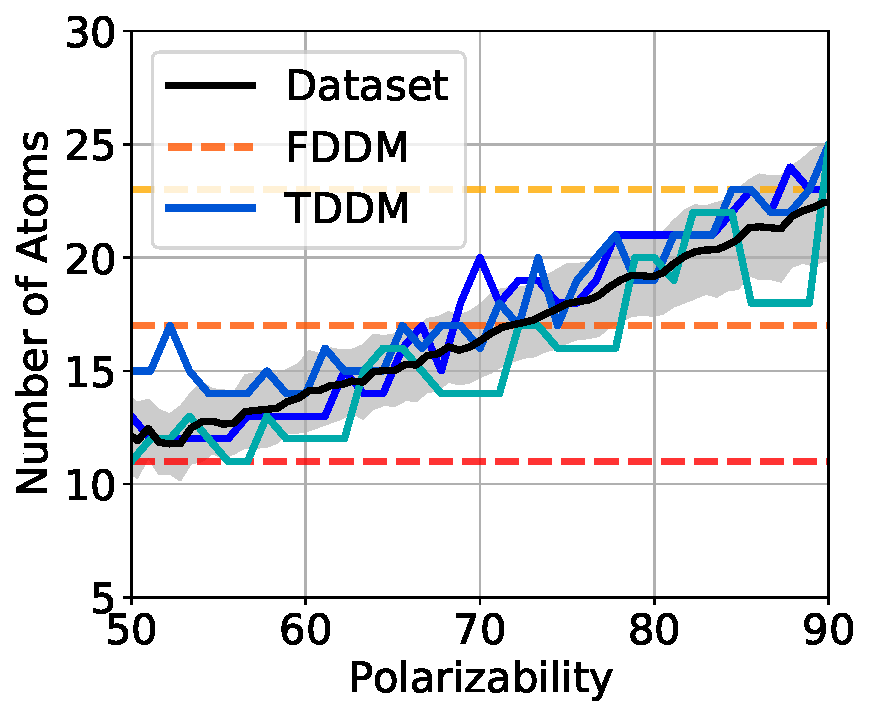
\includegraphics[width=0.45\textwidth]{figs/tddm/polarizability_vs_num_atoms.pdf}
    \caption{Plot of the number of atoms generated by our jump diffusion model against the polarizability (in $\text{Bohr}^3$) conditioned on for three interpolations with fixed random noise. The mean and standard deviation of the number of atoms according to the dataset is also shown. Our FDDM baseline interpolates entirely in a fixed dimensional space hence the number of atoms is fixed for all polarizabilities.}
    \label{fig:tddm-interp_plot}
\end{figure}

\subsubsection{Trans-dimensional interpolation}
\label{sec:mol_interp}
Interpolations are a unique way of gaining insight into the effect of some conditioning parameter on a dataset of interest.
To create an interpolation, a conditional generative model is first trained and then sampled with a sweep of the conditioning parameter but using fixed random noise~\citep{hoogeboom2022equivariant}.
The resulting series of synthetic datapoints share similar features due to the fixed random noise but vary in ways that are very informative as to the effect of the conditioning parameter. 
Attempting to interpolate with an FDDM is fundamentally limited because the entire interpolation occurs in the same dimension which is unrealistic when the conditioning parameter is heavily correlated with the dimension of the datapoint. We demonstrate this by following the setup of \citet{hoogeboom2022equivariant} who train a conditional FDDM conditioned on polarizability. Polarizability is the ability of a molecule's electron cloud to distort in response to an external electric field~\citep{modernphysicalorganicchemistry} with larger molecules tending to have higher polarizability. To enable us to perform a trans-dimensional interpolation, we also train a conditional version of our model conditioned on polarizability. An example interpolation with this model is shown in \cref{fig:tddm-interp}. We find that indeed the size of the molecule increases with increasing polarizability, with some molecular substructures e.g.~rings, being maintained across dimensions.
We show how the dimension changes with polarizability during 3 interpolations in \cref{fig:tddm-interp_plot}. We find that these match the true dataset statistics much more accurately than interpolations using FDDM which first pick a dimension and carry out the entire interpolation in that fixed dimension.

\begin{figure}[t]
    \centering
    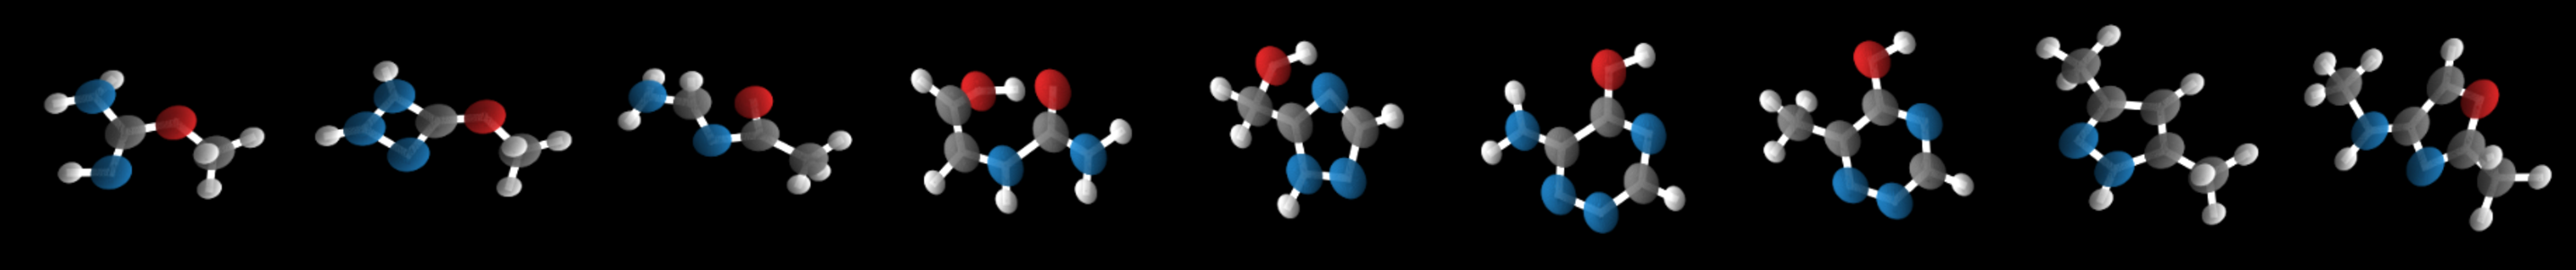
\includegraphics[width=\textwidth]{figs/tddm/small_interp_bright.pdf}
    \caption{Sequence of generations for linearly increasing polarizability from $39 \, \text{Bohr}^3$ to $66 \, \text{Bohr}^3$ with fixed random noise. Note how molecular size generally increases with polarizability and how some molecular substructures are maintained between sequential generations of differing dimension. For example, between molecules 6 and 7, the single change is a nitrogen (blue) to a carbon (grey) and an extra hydrogen (white) is added to maintain the correct valency.}
    \label{fig:tddm-interp}
\end{figure}



\subsection{Video}

We finally demonstrate our model on a video modelling task. Specifically we model the RoboDesk dataset~\citep{tian2023control}, a video benchmark to measure the applicability of video models for planning and control problems. The videos are renderings of a robotic arm~\citep{kannan2021robodesk} performing a variety of tasks including opening drawers and moving objects.
We first train an unconditional model on videos of varying length and then perform planning by using diffusion guidance to generate videos conditioned on an initial starting frame and a final goal frame \cite{janner2022diffuser}. The planning problem is then reduced to ``filling in'' the frames in between. Our trans-dimensional model automatically varies the number of in-filled frames during generation so that the final length of video matches the length of time the task should take, whereas the fixed dimension model relies on the unrealistic assumption that the length of time the task should take is known before generation.

We model videos at $32 \times 32$ resolution and with varying length distributed uniformly between $2$ and $35$ frames. For the network backbone, we use a UNet adapted for video \cite{harvey2022flexible}. In contrast to molecular point clouds, our data is no longer permutation invariant hence $A_t^\theta(\yadd, i | \mX_t)$ includes a prediction over the location to insert the new frame. Also, since each component of a datapoint is an entire video frame, we found that it was difficult to obtain good results when adding components at $t$ far from $T$ with any simple parameterisation of $A_t^\theta(\yadd, i | \mX_t)$. We therefore adapt our diffusion process to be non-isotropic, meaning that different components (frames) have differing amounts of noise applied. This means that, whenever a component is added, a very noisy version of its values can be initialised by $A_t^\theta(\yadd, i | \mX_t)$ even if there is less noise added to the presently-existing components. For simplicity, our formalisation of this, as detailed in \cref{sec:tddm-ExperimentDetails}, removes all noise from each existing component before adding new components. As such, while we describe this model in the jump diffusion framework, it can be equivalently interpreted as an any-order autoregressive model~\citep{shih2022training} that uses a conditional diffusion model within each sampling stage. 

We evaluate our approach on three planning tasks, holding stationary, sliding a door and pushing an object. An example generation conditioned on the first and last frame for the slide door task is shown in \cref{fig:tddm-video_example}, with the model in-filling a plausible trajectory. We quantify our model's ability to generate videos of a length appropriate to the task in \cref{tab:video_results} finding on all three tasks we generate a more accurate length of video than FDDM which is forced to sample video lengths from the unconditional empirically observed length distribution in the training dataset. Full experimental details are provided in \cref{sec:tddm-ExperimentDetails}.

\definecolor{videored}{HTML}{f00606}
\definecolor{videoblue}{HTML}{4b4bfc}

\begin{figure}[t]
    \centering
    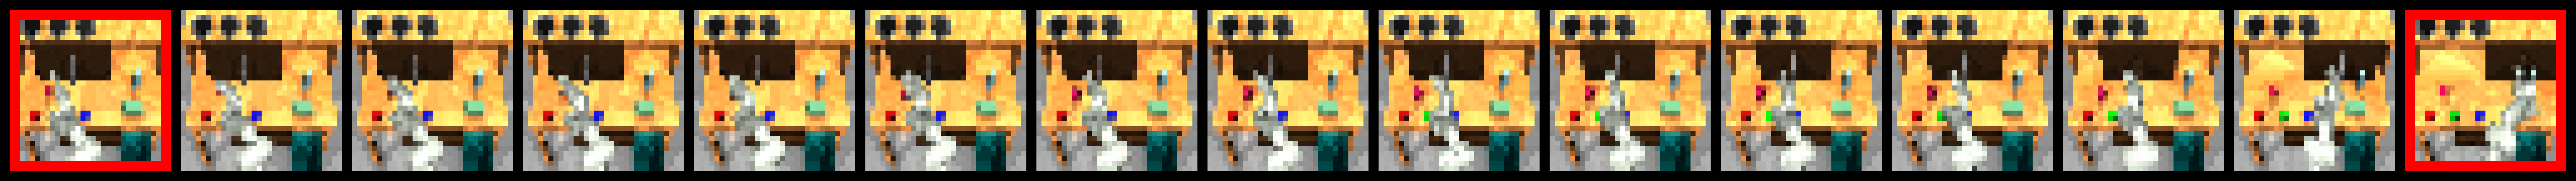
\includegraphics[width=\textwidth]{figs/tddm/21-1-padded_red_big.png}
    \caption{A sample for the slide door task conditioned on the first and last frame ({\color{red} highlighted}).}
    \label{fig:tddm-video_example}
\end{figure}

\begin{table}[t]
     \centering
   \caption{Evaluation of videos generated conditioned on first and last frame. We report the mean absolute error in the number of frames sampled
   for three planning tasks. Standard deviations are estimated over 45 samples.}
   \begin{tabular}{@{}lcccc@{}}
     \toprule
     Method & Stationary ($\downarrow$) & Slide Door ($\downarrow$) & Push Object ($\downarrow$) & Average ($\downarrow$)   \\ \midrule
     FDDM & $14.16 {\scriptstyle \pm 1.41}$ & $13.39 {\scriptstyle \pm 1.34}$ & $17.06 {\scriptstyle \pm 1.47}$ & $14.87$ \\
     TDDM & $\mathbf{9.70 {\scriptstyle \pm 0.99}}$ & $\mathbf{11.47 {\scriptstyle \pm 0.74}}$ & $\mathbf{15.43 {\scriptstyle \pm 0.90}}$ & $\mathbf{12.2}$ \\ \bottomrule
   \end{tabular}
   \label{tab:video_results}
\end{table}


\section{Discussion}
We have presented jump diffusion models for trans-dimensional generative modelling, and shown that flexible generative modelling is possible even when we are drawing samples of variable dimensionality. We have demonstrated this on both molecular and video data. On molecular data, there are also many further directions worth exploring such as generating larger molecules or generating molecules conditioned on what other molecules they interact with, a task of great interest in drug discovery~\citep{hoogeboom2022equivariant}. The video data gives a proof in principle that the visual planning task discussed previously can be made robust to goals that will take an unknown time to achieve. Additionally, the trans-dimensional generative models we presented can in principle be applied to any domain with varying-dimensional data. Ones in which objects are explicitly represented, or tracked, would be prime targets with relevance to the vision domain~\citep{luo2021multiple,niedoba2024diffusion}. 